\begin{figure}[h!]
    \begin{subfigure}{.5\textwidth}
    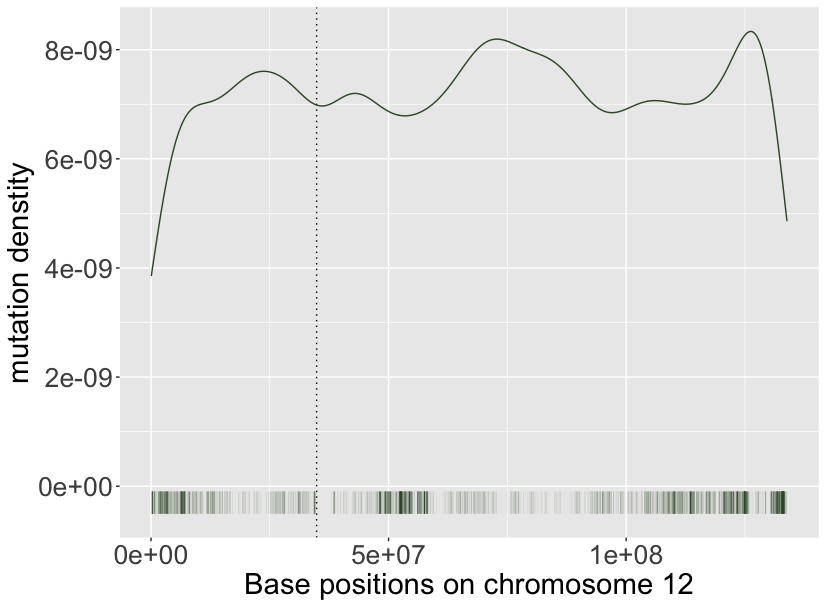
\includegraphics[width=\linewidth,height=0.7\textwidth]{graphics/mutdistribution_Breast-AdenoCa.png}
    \caption{Breast-AdenoCa}
    \end{subfigure}
    ~
    \begin{subfigure}{.5\textwidth}
    \includegraphics[width=\linewidth,height=0.7\textwidth]{graphics/mutdistribution_.png}
    \caption{CNS-Medullo}
    \end{subfigure} \\
    \vspace{0.5cm}
    
    \begin{subfigure}{.5\textwidth}
    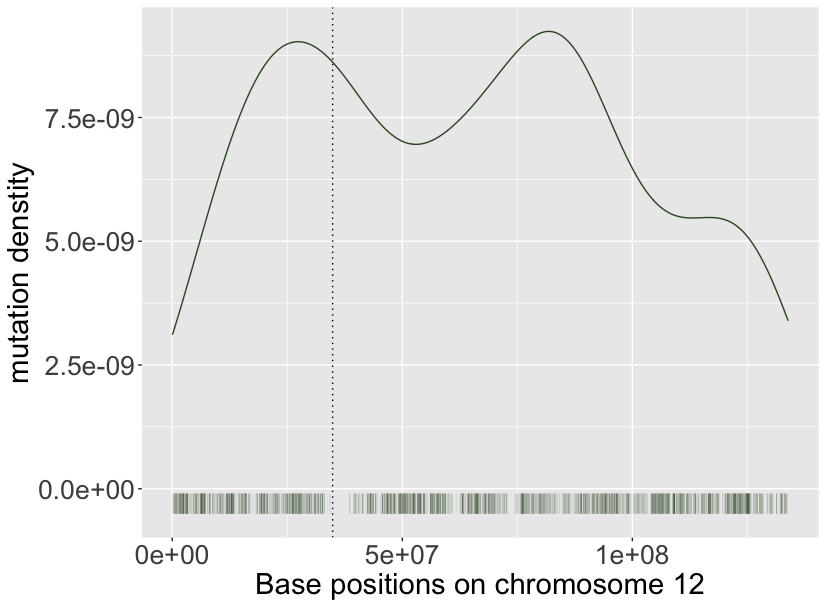
\includegraphics[width=\linewidth,height=0.7\textwidth]{graphics/mutdistribution_CNS-PiloAstro.png}
    \caption{CNS-PiloAstro}
    \end{subfigure}
    ~
    \begin{subfigure}{.5\textwidth}
    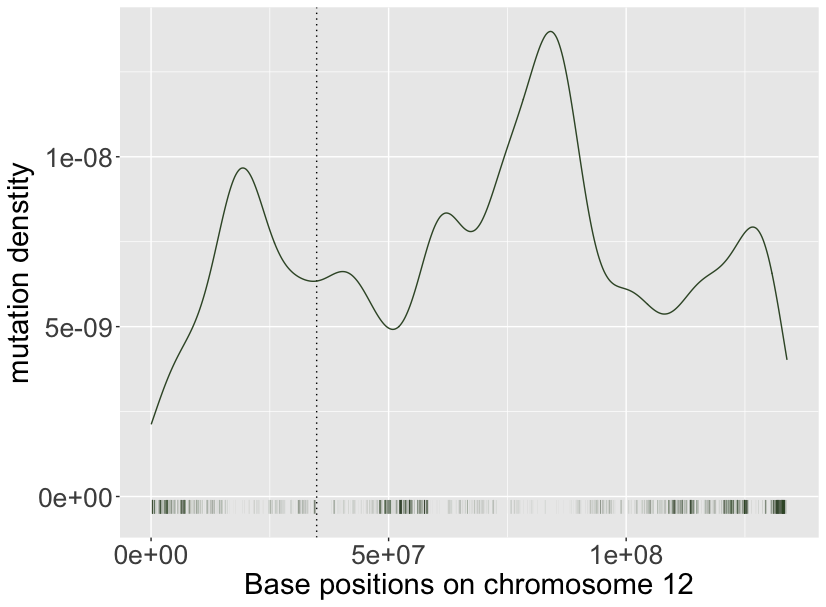
\includegraphics[width=\linewidth,height=0.7\textwidth]{graphics/mutdistribution_Lymph-BNHL.png}
    \caption{Lymph-BNHL}
    \end{subfigure} \\
    
    \begin{subfigure}{.5\textwidth}
    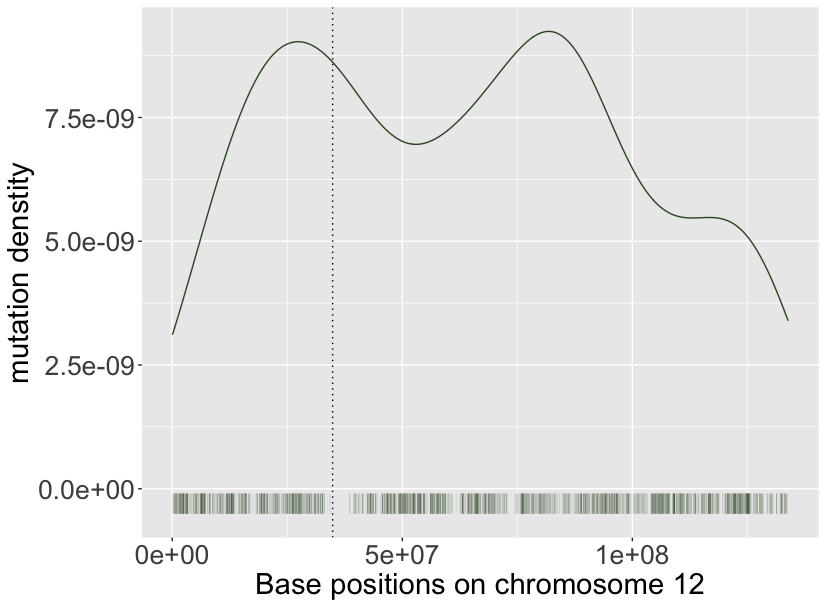
\includegraphics[width=\linewidth,height=0.7\textwidth]{graphics/mutdistribution_CNS-PiloAstro.png}
    \caption{CNS-PiloAstro}
    \end{subfigure}
    ~
    \begin{subfigure}{.5\textwidth}
    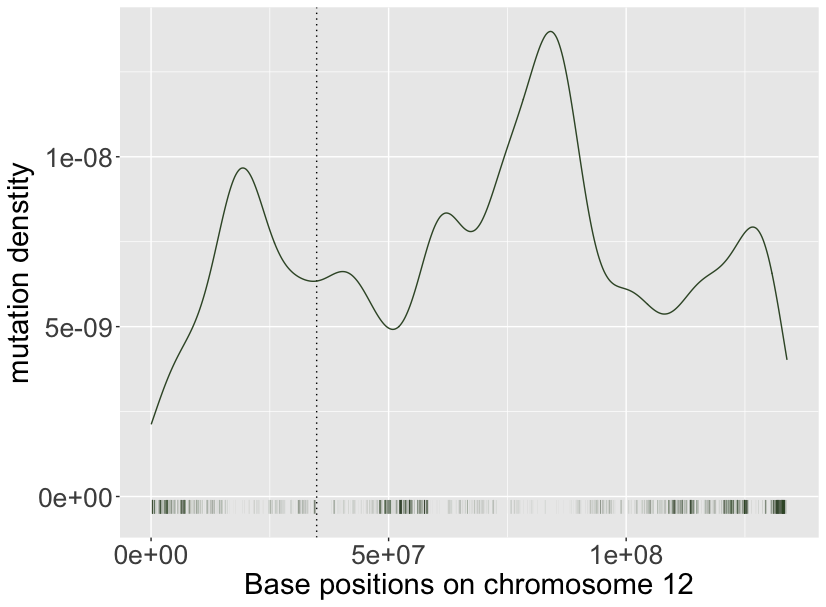
\includegraphics[width=\linewidth,height=0.7\textwidth]{graphics/mutdistribution_Lymph-BNHL.png}
    \caption{Lymph-BNHL}
    \end{subfigure} \\
    
    \begin{subfigure}{.5\textwidth}
    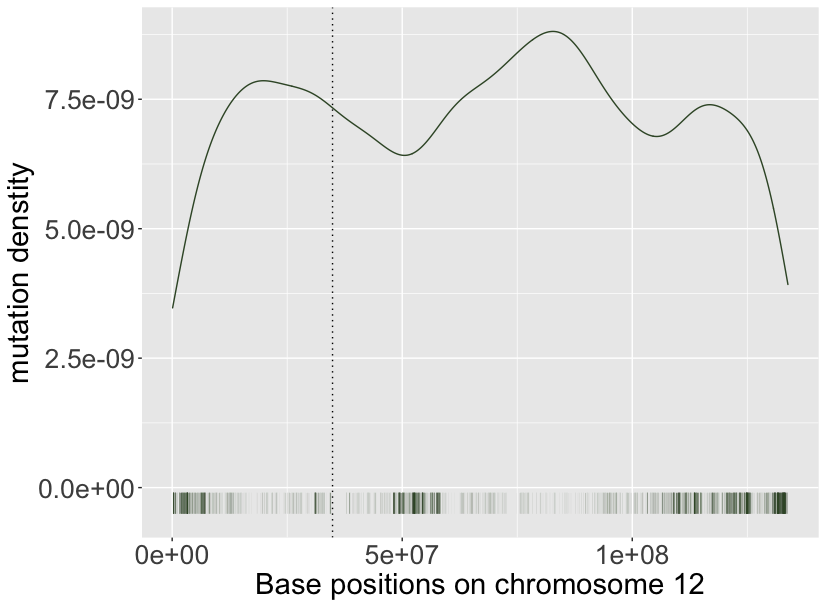
\includegraphics[width=\linewidth,height=0.7\textwidth]{graphics/mutdistribution_Panc-Endocrine.png}
    \caption{Panc-Endocrine}
    \end{subfigure} 
    ~
    \begin{subfigure}{.5\textwidth}
    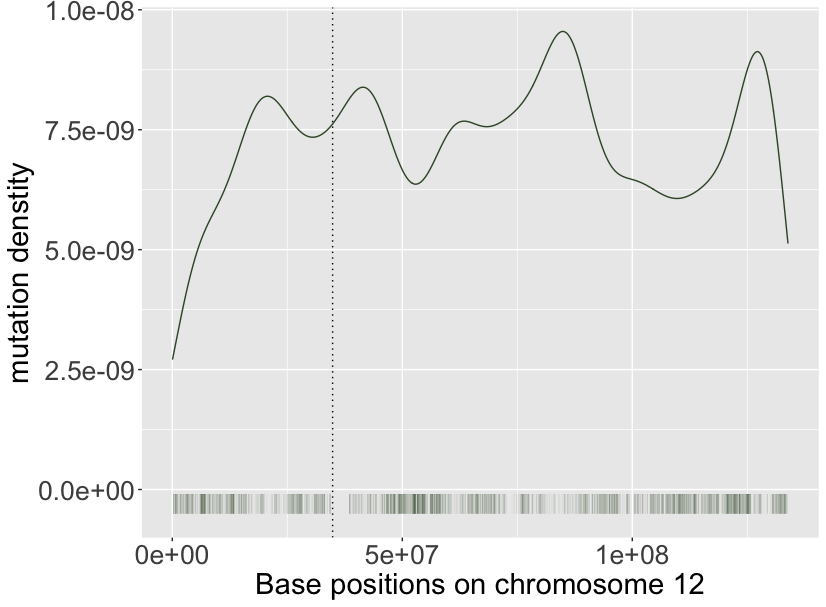
\includegraphics[width=\linewidth,height=0.7\textwidth]{graphics/mutdistribution_Prost-AdenoCA.png}
    \caption{Prost-AdenoCA}
    \end{subfigure} \\

    \caption{\textbf{Mutations tend to be found in closed chromatin regions.} Different cancers differ in the distribution of mutations across the genome. Here chromosome 12 is shown. Other chomosomes are available upon request. The green bar below the x-axis indicates hypersensitivity regions, the gap indicates closed chromatin regions. The vertical dotted line indicates the position of the centromere.}
    \label{fig:apdx_mutation_density}
\end{figure}